\documentclass[12pt]{article}

\usepackage{fullpage}
\usepackage{graphicx, rotating, booktabs} 
\usepackage{times} 
\usepackage{natbib} 
\usepackage{indentfirst} 
\usepackage{setspace}
\usepackage{grffile} 
\usepackage{hyperref}
\usepackage{adjustbox}
\setcitestyle{aysep{}}


\singlespace
\title{
\textbf{Reassessing the Public Goods Theory of Alliances}
	}
\author{Joshua Alley\footnote{Graduate Student,
Department of Political Science, Texas A\&M University.}}
\date{{\normalsize \today}}

\bibliographystyle{apsr}

\begin{document}

\maketitle 

\doublespace

\begin{abstract}
The public goods model of alliances exerts a large influence on scholarship and policy, but it has not received sufficient empirical scrutiny. 
Prior tests of the public goods argument suffer from a mix of identification and generalizability problems. 
This study addresses those limitations by testing two implications of the public goods model. 
First, I test whether state size modifies the impact of increasing allied capability on growth in military spending. 
Then I estimate the association between a states share of alliance capabilities and growth in military spending for 285 offensive and defensive alliances. 
The results from my analysis contradict the expectations of the public goods model. 
Therefore, the argument that alliances provide a public good and generate free-riding incentives should be treated with more skepticism. 

\end{abstract} 



%----------------------------------
\section{Introduction}



\citet{OlsonZeckhauser1966} argue that international alliances generate a collective action problem. 
According to their theory, security from an alliance is a public good, which allows smaller alliance participants to ``free ride'' on the contributions of larger members. 
Free-riding is reflected in lower defense burdens--- states allocate a lower share of their resources to defense.
This view of alliances and defense effort is quite influential in scholarship \citep{Walt1990, Mearsheimer1994, SandlerHartley2001, Garfinkel2004, Walt2009, Barrett2010}. 
In addition, policy discussions of alliances rely on the idea of collective action.
Commentators and American policymakers often refer to allied ``free-riding.'' 
Thinking of alliance security as a public good and beset by collective action problems, generates fear that the US is ``being taken advantage of'' by junior partners. 


US policymakers make frequent use of free-riding and disproportionate contributions to the common good to criticize lackluster allied defense expenditures.  
For example, Barack Obama complained in 2016 that ``Free riders aggravate me'' and US allies ``have to pay your fair share.'' 
Donald Trump has implied the US will not protect allies who spend too little on defense. 
Such exhortations go back to the Eisenhower administration \citep{Lanoszka2015}.


In US alliance politics, the North Atlantic Treaty Organization (NATO) is the epicenter of free-riding discussions. 
Following Olson and Zeckhauser's emphasis on the defense burden, accusations of free-riding emphasize how NATO allies spend a lower share of their income on defense than the US. 
Pundits and policy makers now employ spending 2\% of GDP on defense as a threshold for adequate effort.
NATO members made a formal commitment to meet this spending target in 2014.\footnote{
\href{https://www.economist.com/graphic-detail/2017/02/16/military-spending-by-nato-members}{In 2017 only four NATO members besides the US met the 2\% threshold.}}  


The failure of many NATO members to bear an adequate defense burden is presented as evidence of free-riding. 
US policymakers assert low allied defense burdens are an inadequate contribution to collective defense. 
European allies reject this characterization of their defense spending, arguing they make other crucial contributions to common defense. 
Academic studies echo this debate about free-riding.  
Scholars have spent decades arguing over whether defense burdens of NATO members reflect free-riding \citep{SandlerForbes1980, Palmer1990, GatesTerasawa1992, SandlerHartley2001, Lanoszka2015, PluemperNeumayer2015}.


Olson and Zeckhauser's argument shaped a generation of policy and scholarly debate about alliances and defense spending. 
But 52 years after the publication of ``An Economic Theory of Alliances,'' we have limited evidence for or against their empirical predictions. 
Therefore, it is still unclear whether the public goods approach to alliances is a good model of alliance politics. 
The lack of reliable evidence is the consequence of two problems. 


First, many empirical estimates of defense burdens within alliances are unidentified.
Olson and Zeckhauser's measures of the defense burden and state size create an identification problem. 
They estimated correlations between military spending as a share of national income and national income.
While this approach is widely emulated, it places GDP on both sides of the equation.
Therefore, most empirical models of the public goods theory are unidentified.


In Olson and Zeckhauser's test, changes in GDP impact the independent and dependent variable. 
There is a deterministic component in the relationship between GDP and the defense burden--- changes in GDP shift the defense burden.\footnote{
The only exception occurs when military spending changes in such a way that defense spending's share of GDP is unchanged. Such changes are possible, but highly unlikely.}  
Moreover, ratio dependent variables such as military expenditures as a share of GDP often generate spurious results \citep{Kronmal1993}. 


One noteworthy paper addresses the identification problem, but may not produce generalizable findings. 
\citet{PluemperNeumayer2015} examine how changes in spending by NATO members respond to US and Soviet spending. 
In their framework, unresponsiveness to US and Soviet military spending is evidence of free riding by non-US NATO members.
They find no correlation between NATO member size and free-riding, which they argue contradicts Olson and Zeckhauser.\footnote{
However, they do not include the United States in their sample, which omits a crucial data point for testing the size argument. Given the focus on responses to US spending, this decision is understandable.}


% So what is the problem here? 
\citet{PluemperNeumayer2015} focus on NATO reflects the other major research design shortcoming--- a lack of generalizability. 
Most studies focus on NATO and most evidence suggests NATO members spend less on the military thanks to allied capability \citep{GeorgeSandler2017}.
But NATO is an unusually capable and durable treaty, making it a difficult case to draw general conclusions from. 


% by the way, it's mostly NATO
We do not know whether the public goods theory of alliances applies to treaties besides NATO. 
My survey of the literature on alliance participation and military spending found six tests of the public goods theory of alliances outside of NATO. 
All six of those studies include GDP in the independent and dependent variable. 
These tests of the public goods theory outside of NATO are unreliable. 


% I'm not the first one to address this theory: first comprehensive empirical evidence
Other scholars have questioned and revised the underlying logic of the public goods theory of alliances \citep{Palmer1990, SandlerHartley2001}.  
But theoretical revisions are premature without clear evidence a parsimonious public goods model is inappropriate. 
We should not rule out an intuitive public goods theory without evidence it makes inaccurate predictions.
\footnote{Findings of no correlation between GDP and the defense burden have the same identification problem.} 
Moreover, popular and policy discussions of alliance politics implicitly depend on the public goods model of alliances. 
Policy efforts to address lower military spending could fail if they are based on an inaccurate model of alliance politics. 


In this paper, I address the identification and generalizability issues in two novel tests the public goods model of alliances.  
Both research designs examine how alliance participant size shapes growth in military spending. 
The first design uses a conventional panel data model with an aggregate measure of alliance participation. 
I interact state size and changes in allied spending examine whether states reduce military expenditures as a result of increasing allied spending, and if reductions diminish with greater state size. 
The second design employs a Bayesian model to estimate the association between treaty contribution and growth in military spending for individual alliances. 
Neither approach finds evidence to match Olson and Zeckhauser's prediction that greater size requires more military spending. 


The paper proceeds as follows.
First, I summarize the public goods theory of alliances and two predictions of its logic.
Then, I describe the results of a panel-data test of the first prediction.
The third section tests the second prediction with a Bayesian multilevel model. 
The final section assesses aggregate support for the public goods logic, as well as implications for scholarship and policy. 



\section{The Public Goods Theory of Alliances}

% summarize argument
Why might alliances suffer from a public goods problem? 
The aggregate military capability of an alliance provides security for members. 
Because a treaty cannot exclude members without undermining its purpose, security is a public good. 
Treaty members receive security regardless of their individual contribution. 
Therefore states have incentives to rely on other members to contribute military capability to the treaty. 


In this model, states contribute to an alliance by investing in their military. 
Olson and Zeckhauser expect larger members of the alliance will bear a higher defense burden, because these states value defense from the alliance more. 
Smaller alliance members rely on the contributions of larger partners for security and bear a lower defense burden.
As a result, smaller states exploit larger alliance participants by free riding. 


% Military spending as outcome
Olson and Zeckhauser expect that within alliances, state size will be positively correlated with the percentage of national income spent on defense.
Size discrepancies among members allow smaller states to free-ride on larger partners. 
Using military spending as a share of GDP is likely to generate spurious results, so I do not test this exact prediction. 
Instead, I test two slightly different implications of the public goods theory of alliances. 


The first prediction aggregates participation in multiple alliances into a single factor. 
A public goods logic uses state size and allied capability to predict how states allocate resources to defense. 
If Olson and Zeckhauser's argument is correct, small states should lower growth in military spending in response to greater allied military spending. 


A small state will tend to rely on their allies for security. 
Greater allied capability increases the ability of small states to rely on allies for security. 
Thus greater allied capability will reduce growth in military spending for small states.

 
Larger states will be less responsive to increased allied capability. 
These states value security from their alliances more, and will spend more on the military to contribute to the treaty. 
For large states, greater allied capability will reflect more obligations, not opportunity to free-ride.


This implies a conditional relationship between allied spending, state size, and defense expenditures. 
Small states should respond to greater allied capability by reducing defense spending. 
But as state size increases, the negative effect of allied capability on defense spending will diminish. 


\begin{quote}
\textsc{Hypothesis 1}: The marginal effect of changes in allied military spending on annual growth in military spending will be negative for small states, and increasing in state size. 
\end{quote}


A different prediction emphasizes what states contribute to individual treaties. 
State size and allied capability determine how much a state contributes to each alliance.
If size could be relative to other alliance members, rather than absolute, the same state could make heterogeneous commitments to different treaties. 
As a result, treaties will have heterogeneous effects on members' defense spending, and greater contributions will require more defense spending. 

 
The public goods model argues that larger members of a treaty value security more and are thus more willing to invest in military capability.
If this is the case, greater treaty contribution should increase military spending. 
Higher growth in spending maintains security from alliance treaties. 
Among treaty members, states with a larger share of allied military capabilities should spend more on the military, all else equal. 


\begin{quote}
\textsc{Hypothesis 2}: For individual alliance treaties, increasing treaty contribution will be positively associated with annual growth in military spending. 
\end{quote}


Treaties with a positive correlation between contribution and military spending conform to Olson and Zeckhauser's expectations. 
No correlation indicates larger alliance members are not increasing military expenditures.
A negative correlation between treaty contribution and military spending implies larger members decrease spending. 
Therefore, I will examine how many alliances have a positive correlation between treaty contribution and military spending.  


I now test these two predictions using a corresponding research design in a sample of all non-microstates from 1816 to 2007.\footnote{Including states with small GDP values makes estimating the interaction in Hypothesis 1 difficult. These observations create a large range of the modifying variable with no support for interactive estimates.}
State-year observations are the unit of analysis in both tests. 
The next section examines Hypothesis 1 by interacting changes in total allied spending and GDP.
This approach aggregates multiple treaties into a single measure of alliance participation. 


\section{Testing Hypothesis 1}

To test Hypothesis 1, I employ conventional measures of state size and alliance participation. 
Olson and Zeckhauser use GDP as a proxy for state size, so I constructed a measure of GDP using data from the Maddison Project \citep{Boltetal2018}. 
I then take the natural log of GDP to address the variable's skewed distribution. 
I measure changes in allied capability by differencing the military spending of all defensive or offensive alliance partners of a state.\footnote{This also corresponds to one key independent variable in the best test of the public goods logic to date \citep{PluemperNeumayer2015}.} 
All alliance membership data comes from the Alliance Treaty Obligations and Provisions (ATOP) data \citep{Leedsetal2002}.  


Growth in military spending is the dependent variable \citep{SingerCINC1988}. 
Olson and Zeckhauser use defense spending as a share of GDP as their dependent variable, which is the source of identification problems in previous research \citep{Kronmal1993, PluemperNeumayer2015}. 
I use spending growth instead of the defense burden because this measure addresses helps give a sense of changes in defense budgets with a lower risk of produce spurious inferences. 
Annual growth in spending is the change in military spending as a share of the previous year's budget. 
Measuring growth in spending gives a sense of the burden of changes in military spending, matching Olson and Zeckhauser's emphasis on how alliance participants allocate resources to the military.
Positive growth in spending implies an expanding defense budget.\footnote{Including GDP in the model controls in part for changes in national income.} 


Moreover, using growth in spending mitigates the risk of spurious inferences due to non-stationarity in panel data. 
The log-level of military spending is not mean-reverting in the long panels I use.
A differenced military spending variable has increasing variance over time, as budgets expand and generate larger changes. 
Modeling the DV in levels or changes with a control for the level might create spurious inferences \citep{GrangerNewbold1974}. 


Using growth in military spending as the dependent variable benchmarks changes to budget size. 
This facilitates comparisons across states and years. 
Growth in spending is equal to: 


\begin{equation}
\mbox{Growth Military Spending} = \frac{\mbox{Mil. Ex.}_t - \mbox{Mil. Ex.}_{t-1} }{ \mbox{Mil. Ex.}_{t-1} } = \frac{\Delta \mbox{Mil. Ex.} }{ \mbox{Mil. Ex.}_{t-1} }
\end{equation} 


Because Hypothesis 1 implies a conditional relationship, I interact allied spending and GDP in the following regression model:

\begin{equation} 
y = \beta_1 + \beta_2 \mbox{ln(GDP)} + \beta_3 \mbox{Ally Spend} + \beta_4 \mbox{ln(GDP)} \times \mbox{Ally Spend} + \beta \mathbf{X} + \epsilon
\end{equation}


$\beta_2$ and $\beta_3$ are the constituent terms of the interaction and \textbf{X} is a matrix of control variables with coefficient vector $\beta$.
Hypothesis 1 implies $\beta_2$ should be positive, and $\beta_3$ should be negative. 
The interaction term $\beta_4$ should be positive. 


I estimate this model with a robust regression estimator--- M estimation with Tukey's Biweight function. 
Growth in military spending has heavy-tailed residuals in a regression, so OLS is inefficient \citep{RaineyBaissa2018}. 
Given heavy-tailed residuals, non-linear estimators such as robust regression can outperform OLS. 
Robust regression re-weights observations using the size of the residual, making it less sensitive to large deviations than OLS. 


\textbf{X} contains correlates of alliance participation and military spending. 
I control for international war \citep{Reiteretal2016}, civil war participation \citep{SarkeesWayman2010}, and a count of annual MIDs \citep{Gibleretal2016}. 
Other controls average salient alliance characteristics, including democratic membership \citep{DigiuseppePoast2016} and number of members across a state's alliance treaties.   
Last, I control for regime type, external threat \citep{LeedsSavun2007}, and Cold War years. 


\subsection{Results}


Estimates from this model do not match the expectations of Hypothesis 1. 
\autoref{tab:rreg-res} summarizes results from the robust regression estimator. 
The constituent terms for the log of GDP and changes in allied spending are statistically insignificant. 
The interaction between changes in allied spending and GDP is also statistically insignificant. 


\begin{table}[!htbp] \centering 
\begin{tabular}{@{\extracolsep{5pt}}lc} 
\\[-1.8ex]\hline 
\hline \\[-1.8ex] 
  & Growth Military Spending \\ 
\hline \\[-1.8ex] 
 Change Allied Spending & $-$0.026 \\ 
  & (0.047) \\ 
  & \\ 
 ln(GDP) & 0.0003 \\ 
  & (0.001) \\ 
  & \\ 
 Change Allied Spending $\times$ ln(GDP) & 0.002 \\ 
  & (0.002) \\ 
  & \\ 
 Avg. Alliance Size & 0.0003$^{*}$ \\ 
  & (0.0002) \\ 
  & \\ 
 Avg Alliance Democracy & $-$0.0003 \\ 
  & (0.001) \\ 
  & \\ 
 International War & 0.097$^{***}$ \\ 
  & (0.010) \\ 
  & \\ 
 Civil War Participant & 0.001 \\ 
  & (0.008) \\ 
  & \\ 
 POLITY & $-$0.0001 \\ 
  & (0.0004) \\ 
  & \\ 
 External Threat & 0.043$^{***}$ \\ 
  & (0.011) \\ 
  & \\ 
 Cold War & 0.047$^{***}$ \\ 
  & (0.004) \\ 
  & \\ 
 Constant & 0.026 \\ 
  & (0.030) \\ 
\hline \\[-1.8ex] 
Observations & 9,139 \\ 
Residual Std. Error & 0.157 (df = 9128) \\ 
\hline 
\hline \\[-1.8ex] 
\textit{Note:}  & \multicolumn{1}{r}{$^{*}$p$<$0.1; $^{**}$p$<$0.05; $^{***}$p$<$0.01} \\ 
\end{tabular} 
\caption{Robust Regression Estimates: Association of interaction of allied spending and GDP with growth in military spending 1816-2007.}
\label{tab:rreg-res}
\end{table}


I cannot infer the absence of an interaction from the coefficients alone \citep{BramborClarkGolder2006}. 
\autoref{fig:abs-margins-plot} plots the marginal effect of allied military spending across the range of GDP. 
The marginal effect of allied military spending can only be distinguished from zero for positive values. 
Although the estimated marginal effect is increasing across the range of GDP, at no point are the effects statistically distinguishable. 


\begin{figure}
	\centering
		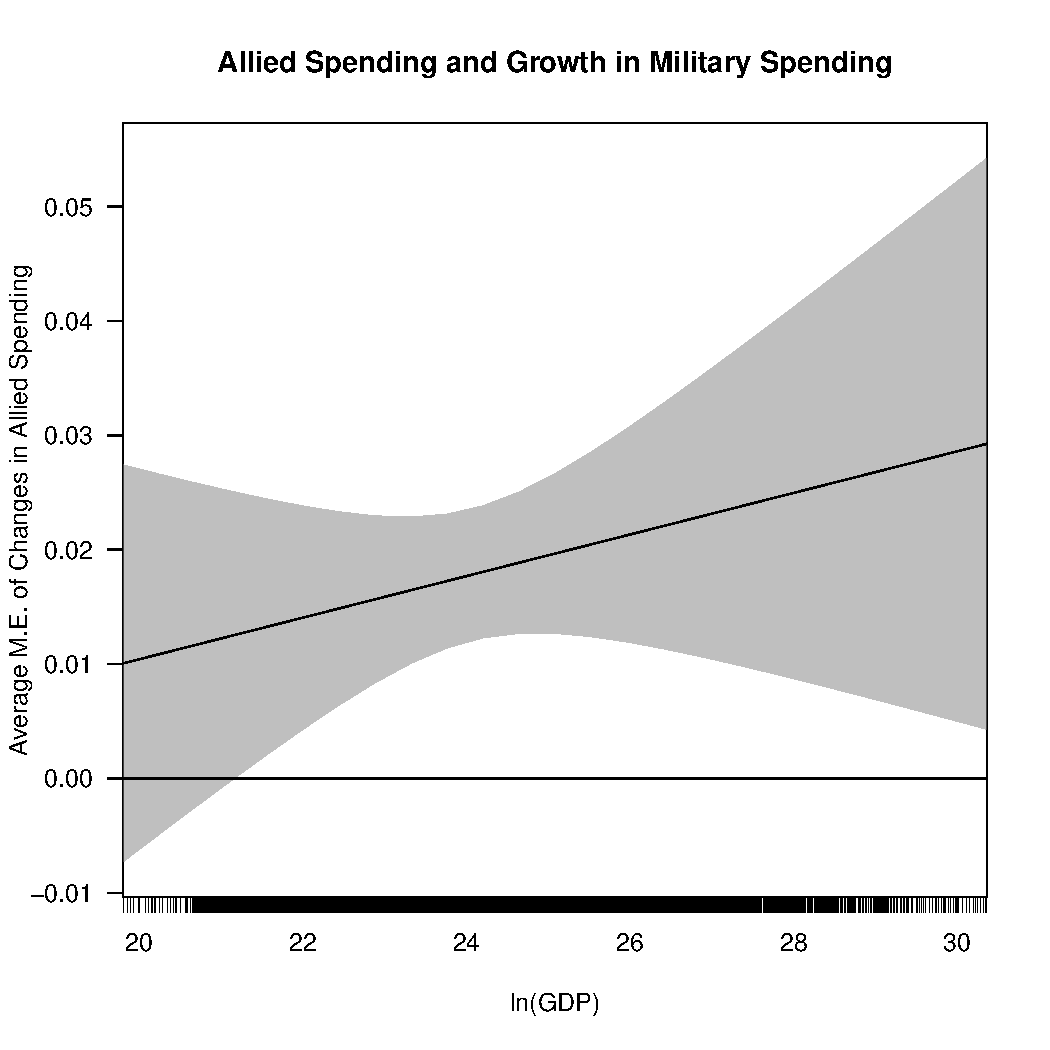
\includegraphics[width=0.95\textwidth]{abs-margins-plot.pdf}
	\caption{Average Marginal Effect of increasing allied military spending on growth in military spending across the range of GDP. Rug plot on x-axis summarizes the distribution of GDP.}
		\label{fig:abs-margins-plot}
\end{figure}


These results do not match the expectations of Hypothesis 1. 
The point estimate is uniformly positive and although the confidence intervals include negative values at very small levels of GDP, the effect is reliably positive for most states. 
There is little evidence increasing allied capability decreases growth in spending for small states. 


These results hold if I replace robust regression with OLS or employ kernel estimation of the interactive relationship \citep{Hainmuelleretal2019}.\footnote{See the appendix for details on these findings.} 
I also estimated a model using states with an alliance as the estimation sample with Heckman two-stage estimator to address non-random selection into alliances. 
Last, I transformed the growth variable using an inverse hyperbolic sine to reduce the heavy-tails in positive and negative values, and used the transformed variable in OLS and robust regressions. 


However, it is possible that aggregating alliance treaties obscures collective action dynamics in individual treaties. 
Olson and Zeckhauser focus on relative size, so states with small GDP can make large alliance contributions if their partner is even smaller. 
The next section examines how often greater treaty contribution increases military expenditures. 


\section{Testing Hypothesis 2}


Testing Hypothesis 2 requires estimating the association between alliance contribution and military spending for each alliance.
For each of the 285 alliances that promise military support,\footnote{ATOP offensive and defensive treaties. Other alliances do not provide security through promises of intervention in conflict. Thinking about the relative contribution to the aggregate capability of a non-aggression pact would be odd, for example.} I estimate a parameter measuring the impact of increasing alliance contribution on military expenditures. 
Bayesian estimation regularizes estimates with many parameters, so I fit the following model using STAN \citep{Carpenteretal2016}.


The full model starts with state-year growth in military spending $y_{it}$.
I model the DV with a t-distribution to account for heavy tails.
$\nu$ is the degrees of freedom parameter--- as $\nu$ increases, the t distribution becomes more like a normal distribution. 


\begin{equation}
y_{it} \sim student_t(\nu, \mu, \sigma) 
\end{equation}


Most of this model follows standard panel data designs.
The expected value of the outcome $\mu_{it}$ depends on a constant $\alpha$, state and year varying intercepts $\alpha^{st}$ and $\alpha^{yr}$ and control variables $X_{it} \beta$. 
In this specification, I include all controls besides the alliance portfolio averages from the first robust regression in $X$.


\begin{equation}
\mu_{it} = \alpha + \alpha^{st} + \alpha^{yr} + \mathbf{X_{it}} \beta + \mathbf{Z_{it}} \gamma 
\end{equation}


The $\mathbf{Z_{it}} \gamma$ term captures the impact of multiple alliances. 
\textbf{Z} is a matrix of state participation in alliances--- columns are alliances, rows are state-year observations. 
If a state is not in an alliance, the corresponding element of the matrix is equal to zero. 
If a state is part of an alliance, the corresponding element of the matrix is equal to a state's military spending as a share of total alliance expenditures. 
The alliance contribution elements of the matrix range from 0 to 1, because some states have no military spending.\footnote{Costa Rica is the best-known example of a state with no military spending, but these cases are highly unusual.} 


\textbf{Z} is a quasi-spatial approach to capturing the impact of participation in multiple alliances.
The ``weight'' of a treaty for growth in military spending depends on how much a state contributes.  
According to Olson and Zeckhauser, greater treaty contribution should increase demand for military spending. 
Lower contribution will lead to reduced growth in spending, because these states can free-ride on their partners.
The correlation between treaty contribution and growth in spending for each alliance is expressed in the $\gamma$ parameters. 


$\gamma$ is a vector of 285 alliance-specific parameters.  
Because \textbf{Z} contains alliance contribution, these coefficients estimate the association between treaty contribution and military spending. 
When a state is not in an alliance, the corresponding $\gamma$ is multiplied by zero, and has no impact. 
Alliance participation only affects military expenditures if a state contributes. 


Each alliance a state is a member of has a separate impact on military spending.
Thus, every alliance estimate holds the impact of other treaties constant. 
A positive $\gamma$ implies that as contribution to the alliance increases, members spend more, as Hypothesis 2 predicts. 
    


\subsection{Results} 


If the public goods theory of alliances is correct, we should observe many positive $\gamma$ parameters. 
Because I employed Bayesian modeling, each $\gamma$ has a posterior distribution.\footnote{See the appendix for a full summary of priors, convergence and model fit.} 
I focus interpretation on the posterior mean and 90\% credible intervals.\footnote{I use 90\% credible intervals because inferences around 95\% intervals can be less stable.}
The posterior mean is the expected value of $\gamma$, while the credible intervals capture uncertainty around that estimate.  


\begin{figure}[htbp]
	\centering
		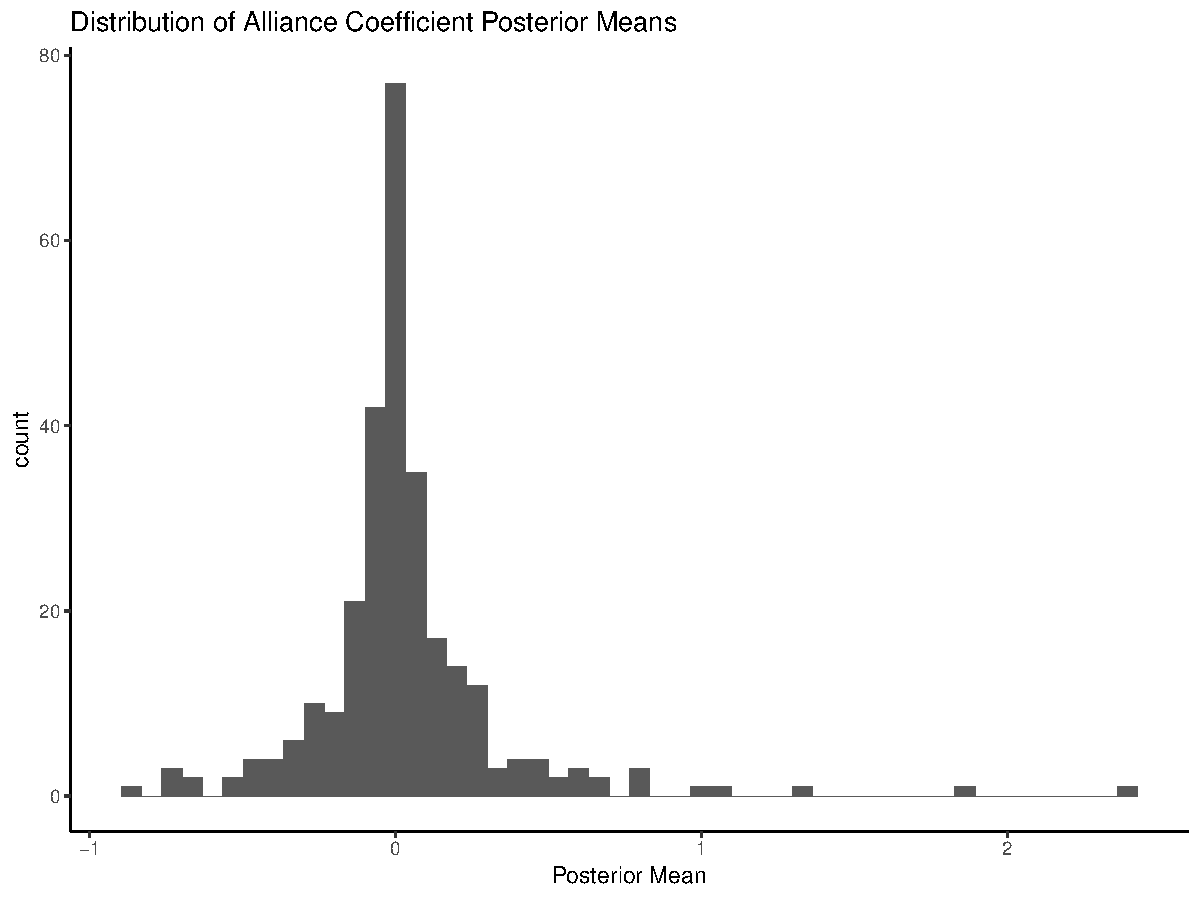
\includegraphics[width=0.95\textwidth]{alliance-coefs-hist.pdf}
	\caption{Posterior mean of association between alliance contribution and military spending in 285 defensive and offensive alliances from 1816 to 2007.}
	\label{fig:alliance-coefs-hist}
\end{figure}


\autoref{fig:alliance-coefs-hist} summarizes the posterior mean of the 285 alliance coefficients. 
Most means are close to zero. 
There are large positive values, but also many large negative values.


147 of 285 alliances have a positive posterior mean. 
138 of 285 alliances have a negative posterior mean. 
The large number of negative values provides some evidence against Hypothesis 2. 


However, the posterior means do not convey when the impact of increasing alliance contribution can be distinguished from zero. 
More positive mass in the posterior of the $\gamma$ parameter for each alliance, adds evidence for Hypothesis 2. 
\autoref{fig:full-post-prob} plots the relative positive and negative posterior probability of each $\gamma$ parameter. 

\begin{figure}[htbp]
	\centering
		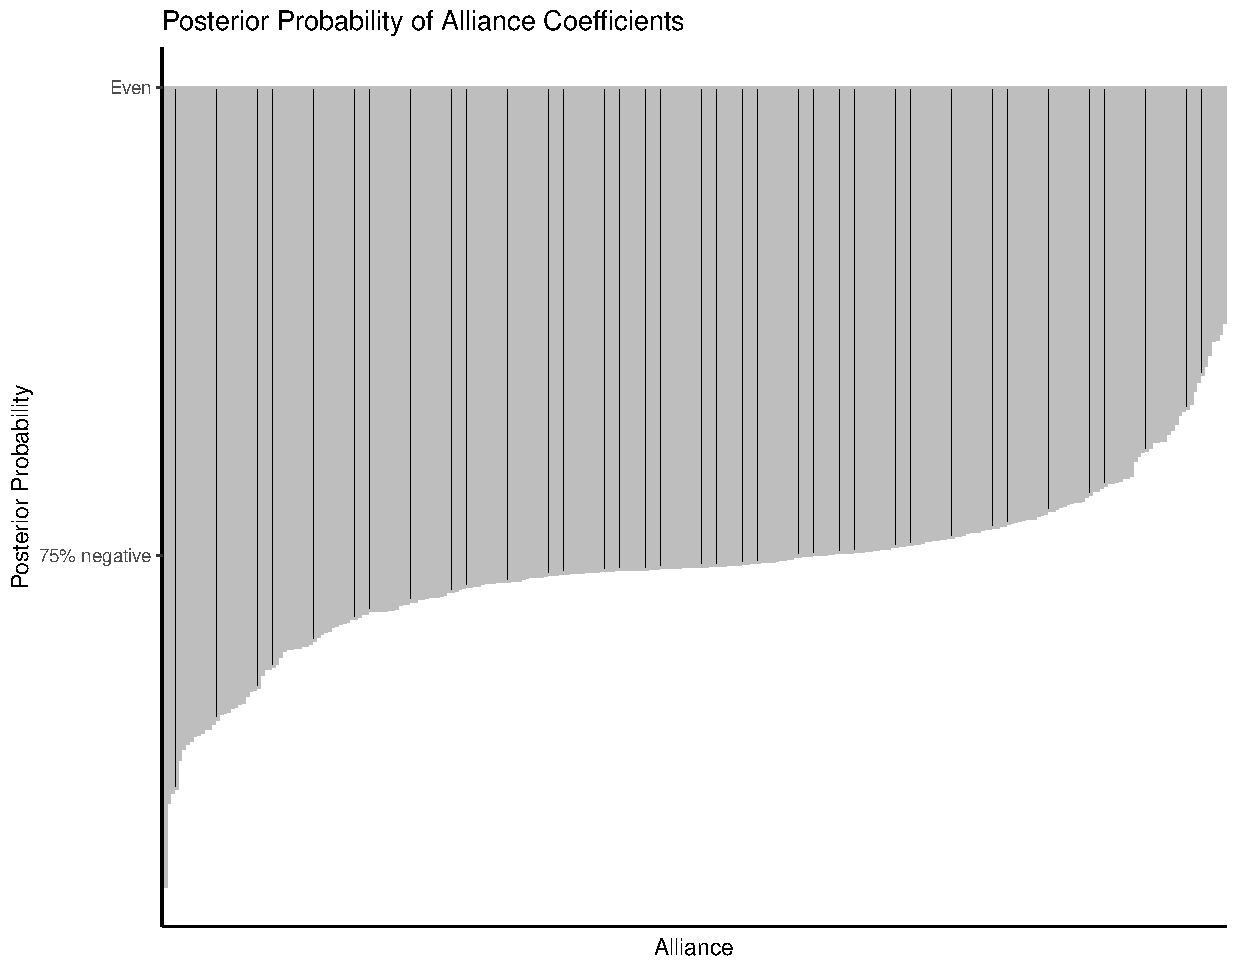
\includegraphics[width=0.95\textwidth]{full-post-prob.pdf}
	\caption{Positive and negative posterior probability of $\gamma$ parameters, sorted by posterior mean. Each column is the relative posterior probability of the effect of increasing contribution for each alliance. Even posterior probability implies 50\% positive and negative posterior mass--- a $\gamma$ parameter with mean 0 and perfectly symmetric uncertainty. Deviations from this add either positive or negative posterior mass.}
	\label{fig:full-post-prob}
\end{figure}


The distribution of positive and negative posterior mass is roughly symmetric, which matches the distribution of posterior means. 
About half of treaties have more positive posterior probability, while the other half have greater negative probability. 
There is little evidence that greater treaty contribution increases military spending in more treaties. 


The credible interval of each $\gamma$ parameter is another source of information about the likely effect of treaty contribution.\footnote{The 90\% credible interval falls between the 5\% and 95\% quantiles of the posterior.} 
\autoref{fig:alliance-coefs-year} plots the $\gamma$ parameter for each alliance against the start year of the treaty.
Points mark the posterior mean. 
The error bars encapsulate the 90\% credible interval.


\begin{figure}[htbp]
	\centering
		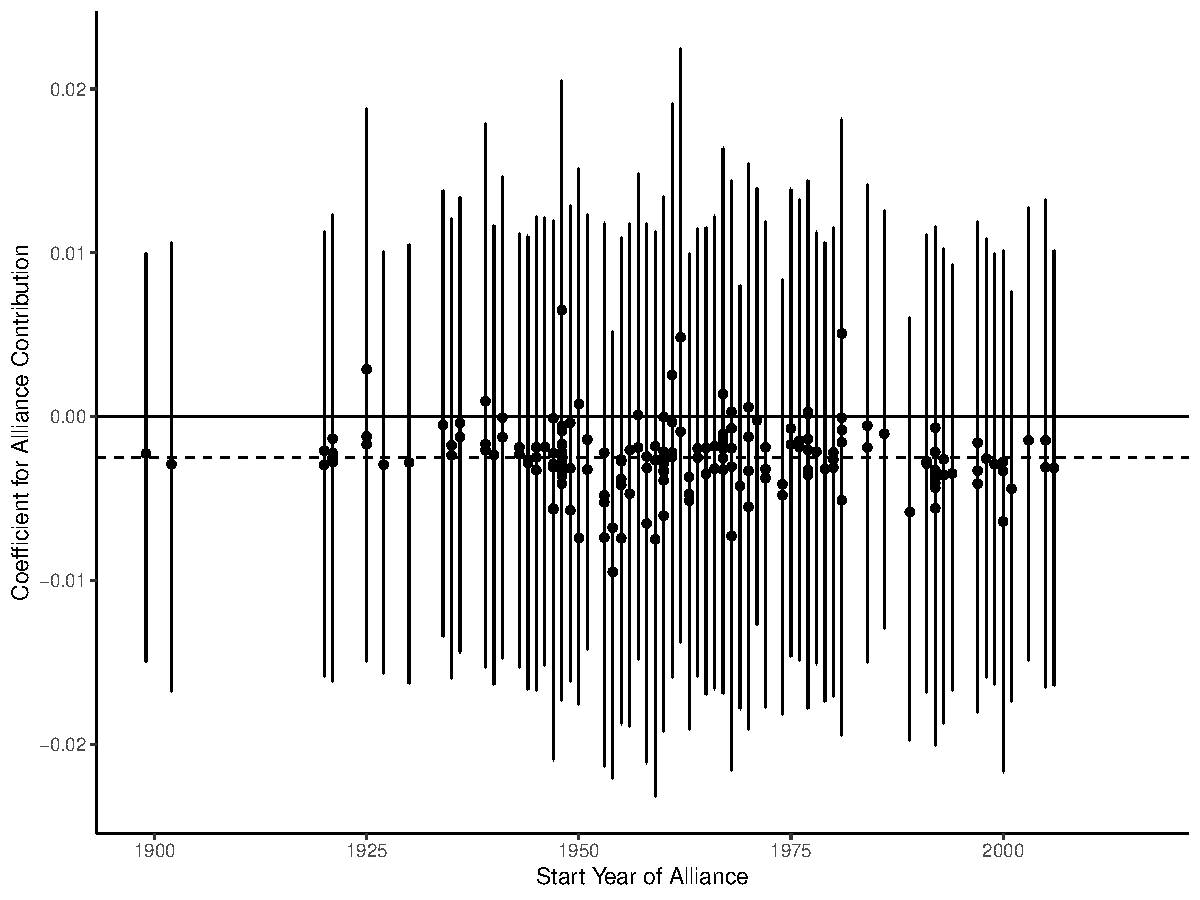
\includegraphics[width=0.95\textwidth]{alliance-coefs-year.pdf}
	\caption{Estimated association between alliance contribution and defense spending in 285 defensive and offensive alliances from 1816 to 2007. Points represent the posterior mean and the error bars cover the 90\% credible interval.}
	\label{fig:alliance-coefs-year}
\end{figure}


Most posterior means are close to zero, so 251 credible intervals include zero. 
There are 16 alliances where the credible interval includes only positive values, as the public goods model predicts. 
That leaves 13 treaties where the credible interval covers only negative values.
16 of 285, or 6\%, is a dismal prediction success rate for Hypothesis 2. 


If we instead calculate the positive and negative posterior probability, as in \autoref{fig:full-post-prob}, we can use 90\% as a threshold. 
In that case, 30 alliances have a $\gamma$ parameter with more than 90\% positive posterior mass. 
Conversely, 22 treaties have a $\gamma$ parameter with more than 90\% negative posterior mass. 
This approach increases the prediction success rate of Hypothesis 2 to 10.5\%. 
 

No approach to examining the association between treaty contribution and military expenditure shows a preponderance of positive coefficients. 
There is no association between treaty contribution and growth in military spending in most alliances.
The 13 negative $\gamma$ parameters imply larger members of those alliances \emph{lower growth in military spending}, which the public goods theory cannot explain. 


These alliances with a high probability of a non-zero $\gamma$ parameter provide additional information. 
I examine these cases in more detail to assess whether collective action is the main issue. 
In \autoref{fig:nonzero-alliance-coefs}, I plot the posterior means of $\gamma$ for all 29 alliances.  
Several of these alliances have a large expected impact on military spending. 


\begin{figure}
	\centering
		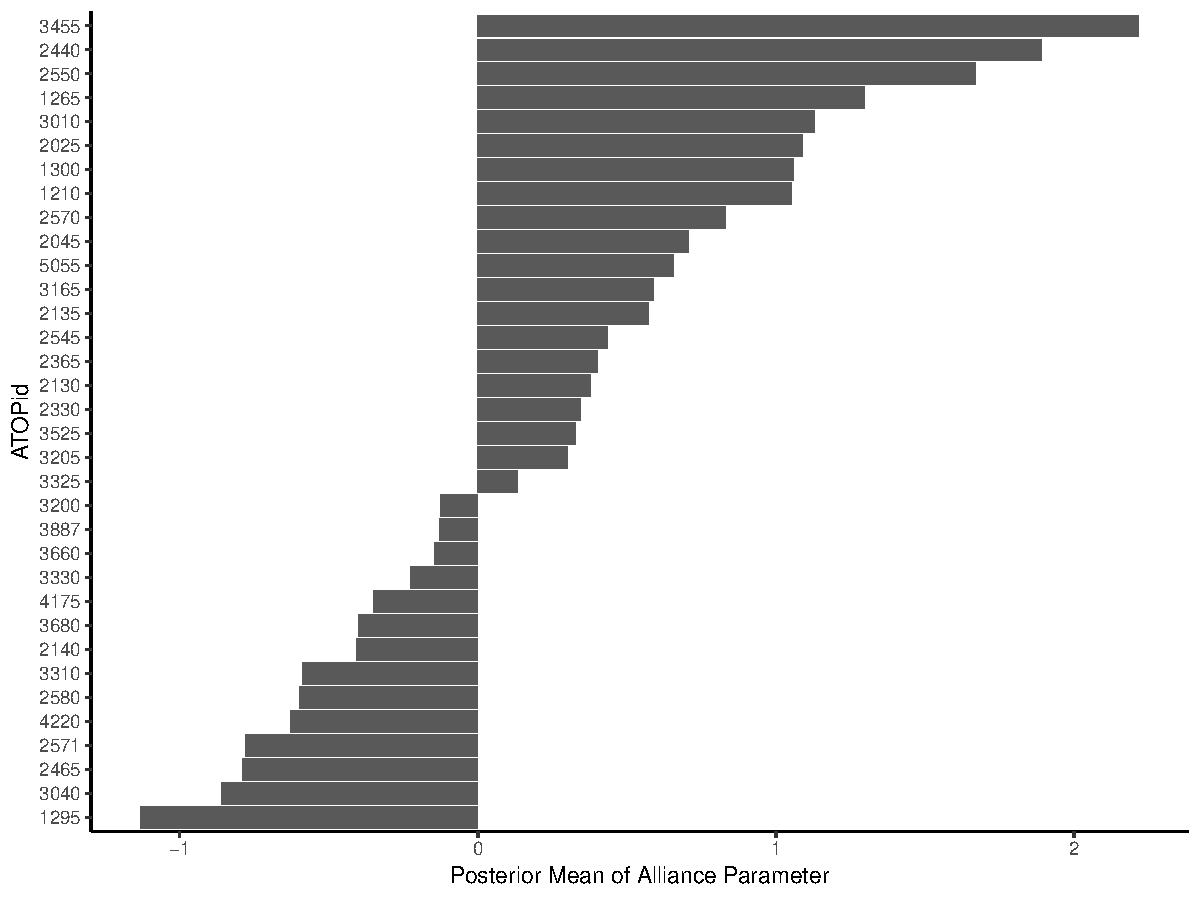
\includegraphics[width=0.95\textwidth]{nonzero-alliance-coefs.pdf}
	\caption{Bar plot of $\gamma$ for alliances where treaty contribution is positively or negatively correlated with military spending. The Y axis is the ATOP project's alliance identifier.}	
	\label{fig:nonzero-alliance-coefs}
\end{figure}

 
The largest positive association between treaty contribution and defense spending growth is the 1961 Defense Pact of the African and Malagasy Union (ATOPID 3455). 
The second largest is an 1866 offensive pact between Italy and Prussia (ATOPID 1265). 
Third largest is an Inter-American Hemispheric defense pact during World War II (ATOPID 3010). 


None of these three cases are obvious examples of free-riding. 
The Defense Pact of the African and Malagasy Union included most Francophone countries. 
The Union changed its functions to focus on economic affairs in 1964, dissolving the defense pact. 
Because the members of this treaty were geographically disparate and depended on France the defense functions of the treaty were weak from the start. 


The Italy-Prussia agreement and the Inter-American Hemispheric defense pact formed immediately before and during war, respectively. 
These treaties are a special cases in Olson and Zeckhauser's model where defense spending is a superior good--- increases in income are spent on defense. 
Larger members spent more because they used the treaty to expand their war-fighting efforts. 


Alliances with large negative $\gamma$ parameters have little in common with a public goods model. 
The largest negative association is an 1870 alliance between Prussia and the UK, signed during the Franco-Prussian war (ATOPID 1295). 
The second largest negative $\gamma$ is a June 1939 alliance between France and Turkey aimed at securing the Mediterranean (ATOPID 2465).
Last, the third most negative $\gamma$ is a 1944 agreement between the US and Portugal, where the Portuguese agreed to help in the Pacific theater. 


These three negative cases suggest states with resource constraints can use alliances to secure their interests and limit spending growth. 
Without a treaty with Prussia to guarantee Belgian neutrality, the UK would have spent more in 1870.
France used the 1939 treaty with Turkey for similar purposes. 
The US formed the 1944 treaty with Portugal to further weaken Japan without exerting more military effort. 
All three alliances structure specific exchanges among members, rather than provide a public good. 


NATO is the best example of collective defense, where other results suggest public goods dynamics are present. 
The estimated $\gamma$ for NATO offers no support for the public goods theory of alliances, however. 
The posterior mean is $-0.07$, and the credible interval ranges from -.30 to .14.  
Greater contribution to NATO is unassociated with growth in military spending. 
This finding corroborates the results of \citet{PluemperNeumayer2015}. 


A few cases may be subject to free-riding. 
The 2006 African Union Non-Aggression and Common Defense Pact (ATOPID 5055) has a positive $\gamma$ that might be explained by free-riding.  
China and North Korea's 1961 alliance (ATOPID 3445) is another possible case--- North Korea might have spent even more on the military without the Chinese alliance. 
Most of the other positive, non-zero $\gamma$ parameters are from treaties formed near international conflict. 


This second set of estimates also provides little support for the public goods theory of alliances. 
In 88\% of alliances, there is no association between treaty contribution and military spending. 
Even cases where treaty contribution is positively correlated with spending may not reflect collective action problems. 

%--- 
% Add discussion section given adequate space. 
%--- 


\section{Conclusion}

% Add paragraph summarizing results
Taking the results from testing Hypothesis 1 and 2 together, there is little evidence for the predictions of the public goods theory of alliances. 
There is little evidence economic size modifies the impact of alliance participation on growth in military spending.
Moreover, there is a clear positive association between treaty contribution and military spending in only 6\% of alliances. 


These findings should increase our skepticism about the public goods model of alliances. 
Although Olson and Zeckhauser's model is simple and intuitive, it lacks explanatory power. 
Better identified empirical models and estimates from multiple treaties show little evidence of collective action problems. 


My results reinforce theoretical skepticism about the public goods model. 
Critiques by \citet{Palmer1990} and \citet{SandlerHartley2001} merit further attention. 
While I have shown little general evidence of collective action problem, pieces of the public goods model may still be useful. 


Some of the results raise additional questions for theoretical work. 
Why do we observe 14 alliances where increasing alliance contributions are associated with reduced spending?
Why is the effect of greater allied spending mostly positive across the range of state size in Model 1? 


Perhaps large and small states use alliances for distinct purposes, so members reap specific gains from treaty participation \citep{Morrow1991}. 
Small states might use alliances to defend their homeland. 
Large states could be more focused on using alliances to defend other states and expand their influence abroad. 


Scholars and policymakers should reassess the way they use ``free-riding'' to describe alliance politics. 
Free-riding is inextricable from a public goods understanding of alliances.
But if key predictions of the public goods model have little empirical support, free-riding is an inaccurate description of reduced defense effort by alliance participants.  
Charges of free-riding may mask exchange between alliance members \citep{Lanoszka2015}. 


Moreover, the idea of free-riding is charged. 
Lots of anecdotal evidence suggests people dislike being taken advantage of, or receiving the ``sucker's payoff.'' 
Policymakers might undermine support for alliances by accusing allies of free-riding. 


We should not completely abandon the public goods model in international politics. 
Other international organizations could suffer from collective action problems.
International environmental regimes and climate change are one noteworthy example.  
Using alliances as exemplars of collective action problems in other international organizations is inappropriate, however. 


Although influential, the public goods model of alliances does not make accurate predictions about state size and defense spending. 
I find little evidence that larger states respond differently to changes in allied capability. 
Few alliances provide public goods in a way that leads to the collective action problem envisaged by Olson and Zeckhauser. 



\singlespace


\bibliography{../../../MasterBibliography} 





\end{document}

